\documentclass[10pt,twocolumn,letterpaper]{article}

% Official WACV 2026 Style (camera-ready)
\usepackage{wacv}
\usepackage{times}
\usepackage{epsfig}
\usepackage{graphicx}
\usepackage{amsmath,amssymb,amsfonts}
\usepackage{booktabs}
\usepackage{multirow}
\usepackage{tabularx}
\usepackage{microtype}
\usepackage[breaklinks,colorlinks,citecolor=blue,linkcolor=red,urlcolor=blue]{hyperref}
\usepackage{cite}
\usepackage{cleveref}

% Camera-ready (final) mode: disables review-only rulers, paper ID, and confidential banner
\wacvfinalcopy

\begin{document}

\title{GauSS: Gaussian Scale-Space Alignment and Refinement for Nano-Scale Tiny Object Detection}

\author{
  Tran Duc Long\thanks{Corresponding author.} \quad
  Phan Thi Thao Tien \quad
  Huynh Huu Hung\thanks{Supervisor.} \\
  University of Science and Technology, The University of Danang \\
  Danang, Vietnam
}

\maketitle

\begin{abstract}
Detecting tiny targets ($2\text{--}20$ pixels) in high-resolution aerial and maritime imagery is constrained by aggressive feature downsampling, which degrades microscopic targets, and by tight computational budgets on unmanned aerial vehicles (UAVs). While incorporating a stride-4 ($P2$) feature map provides higher spatial granularity, naive feature concatenation amplifies sea-surface clutter and sensor noise. We propose \textbf{GauSS} (\textbf{Gau}ssian \textbf{S}cale-\textbf{S}pace Alignment and Refinement), a lightweight module that refines stride-4 ($P2$) representations. GauSS decomposes shallow multi-scale features into complementary frequency bands inspired by discrete Gaussian scale-space operators and uses a spatial router to balance high-frequency detail against structural and contextual guidance. On the TinyPerson benchmark under the standardized TinyPerson Evaluation protocol with isolated train and test splits, GauSS adds $+34{,}666$ parameters ($+1.38\%$) to a YOLO26n-P2 model ($2.55\text{M}$ total). It achieves $12.94\%$ overall $AP_{50}^{\text{all}}$ ($+0.98\text{ pp}$) and $9.50\%$ $AP_{50}^{\text{tiny2}}$ ($8\text{--}12\text{ px}$, $+2.59\text{ pp}$). On an NVIDIA A10G GPU, single-tile latency is $15.19\text{ ms}$ ($65.8\text{ FPS}$), while full-frame inference reaches $16.58\text{ ms}$ ($60.3\text{ FPS}$). We analyze end-to-end tiling latency, report exact scale-bin instance counts, examine design choices, and discuss limitations.
\end{abstract}

\section{Introduction}
\label{sec:intro}

Real-time detection of tiny objects in wide-angle airborne imagery is crucial for maritime search and rescue (SAR), coastal defense, and disaster surveillance~\cite{yu2020tinyperson,zhu2021visdrone,wang2020aitod}. In open-sea search scenarios, a distant person in distress frequently occupies fewer than $20$ pixels in a $1280 \times 1280$ capture, with extreme cases spanning $2\text{--}8$ pixels ($tiny1$ regime). At this microscopic resolution, objects exhibit severe information sparsity: they lack discernible facial or body textures, display low contrast against aquatic environments, and are frequently confounded by reflective wave crests and sensor noise.

\begin{figure}[t]
  \centering
  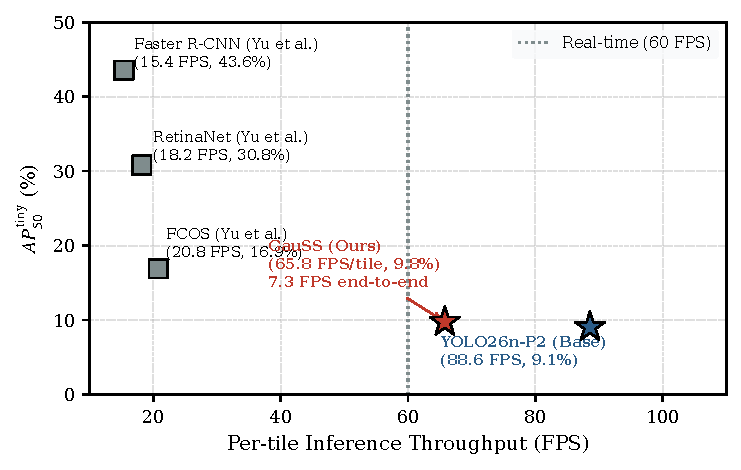
\includegraphics[width=\linewidth]{figures/09_pareto_frontier_tradeoff.pdf}
  \caption{\textbf{Accuracy--Speed Trade-off on TinyPerson}: Accuracy ($AP_{50}^{\text{tiny}}$) versus inference speed (FPS). Faster R-CNN, RetinaNet, and FCOS use heavy backbones ($>32\text{M}$ parameters) and run at $\le 21\text{ FPS}$, whereas \textbf{GauSS} reaches $65.8\text{ FPS}$ per tile ($60.3\text{ FPS}$ full-frame) with $2.55\text{M}$ parameters. Speeds of prior models are taken from published literature and should be interpreted as indicative reference points.}
  \label{fig:pareto_teaser}
\end{figure}

Conventional Feature Pyramid Networks (FPN)~\cite{lin2017fpn} and Path Aggregation Networks (PANet)~\cite{liu2018panet} aggregate features from stride-8 ($P3$) to stride-32 ($P5$). For an object smaller than $8$ pixels, a downsampling stride of 8 reduces its footprint to sub-pixel representations, weakening gradient signals during training. While incorporating a stride-4 ($P2$) feature map preserves spatial granularity -- a strategy now standard in small-object variants of the YOLO family~\cite{ultralytics2026yolo,chao2025bpdyolo} and low-resolution building blocks~\cite{sunkara2022spdconv} -- naive concatenation of shallow features introduces background clutter: shallow layers possess high spatial resolution but lack high-level contextual semantics, generating false positives along reflective wave crests.

Existing tiny-person detectors, such as Scale-Match Faster R-CNN~\cite{yu2020tinyperson} and RetinaNet~\cite{lin2017focal}, tackle this challenge by deploying heavy ImageNet~\cite{deng2009imagenet,russakovsky2015imagenet}-pretrained backbones ($>32\text{--}41\text{M}$ parameters). However, their computational burden makes edge deployment on UAVs challenging. This motivates the central question of this study: can a single-stage nano-scale detector ($<2.6\text{M}$ parameters) maintain competitive microscopic localization while sustaining real-time processing?

To address this challenge, we introduce \textbf{GauSS} (\textbf{Gau}ssian \textbf{S}cale-\textbf{S}pace Alignment and Refinement), a lightweight module that stabilizes and enriches stride-4 ($P2$) features. Drawing inspiration from axiomatic scale-space theory~\cite{witkin1983scale,koenderink1984structure,lindeberg1994scale}, GauSS treats pyramid levels as discrete scale samples. Rather than simple concatenation, GauSS conditions features from three depths: shallow spatial details from Backbone Layer 2 ($C_2$, $64$ channels), lateral neck features from $P3$ ($64$ channels), and dilated contextual guidance from $P4$ ($128$ channels). An adaptive spatial router dynamically weights complementary frequency bands to suppress high-frequency wave artifacts while preserving weak target energy.

We evaluate GauSS on TinyPerson~\cite{yu2020tinyperson} and VisDrone~\cite{zhu2021visdrone}. Under the standardized TinyPerson Evaluation (TOV) protocol ($640 \times 512$ tiled slicing, overlap $100$, global NMS merge), GauSS outperforms the matched YOLO26n-P2 baseline by $+0.98\text{ pp}$ in overall $AP_{50}^{\text{all}}$ ($12.94\%$ vs. $11.95\%$) and by $+2.59\text{ pp}$ in $AP_{50}^{\text{tiny2}}$ ($8\text{--}12\text{ px}$, $9.50\%$ vs. $6.90\%$), reducing $MR_{50}^{\text{tiny2}}$ by $1.58\text{ pp}$. In the ultra-tiny regime ($2\text{--}8\text{ px}$), GauSS achieves $5.18\%$ AP, outperforming the FCOS ResNet-50 reference ($3.39\%$) while requiring $12.5\times$ fewer parameters than heavy multi-stage detectors ($>32\text{--}41\text{M}$ parameters).

Our primary contributions are summarized as follows:
\begin{enumerate}
    \item \textbf{Scale-Space Inspired Architecture}: We design GauSS, a modular refinement unit that structures shallow stride-4 features into discrete frequency bands via learnable separable Gaussian diffusion and an adaptive spatial router ($+34{,}666$ parameters, $+1.38\%$).
    \item \textbf{Controlled Experimental Evaluation}: We establish a rigorous, reproducible scratch-trained baseline (150 epochs) on TinyPerson under the standardized TOV protocol with strictly isolated splits.
    \item \textbf{Transparent Profiling and Analysis}: We provide exact scale-bin instance counts, analyze end-to-end vs. per-tile runtime, examine latency-to-FLOP trade-offs, and report transfer behavior on VisDrone.
\end{enumerate}

\section{Related Work}
\label{sec:related}

\textbf{Tiny and Small Object Detection}: Tiny object detection in aerial and remote-sensing domains~\cite{yu2020tinyperson,wang2020aitod,zhu2021visdrone} presents severe challenges due to information loss and background noise. Yu~\etal~\cite{yu2020tinyperson} introduced TinyPerson alongside Scale Match, demonstrating that standard pre-trained representations suffer from scale mismatch on targets smaller than 20 pixels. Wang~\etal~\cite{wang2021nwd} proposed Normalized Wasserstein Distance (NWD) to replace sensitive IoU metrics for tiny instances. Recent works have explored receptive field learning (RFLA)~\cite{chen2021rfla} and sliding-window slicing techniques such as SAHI~\cite{akyon2022sahi}. However, most established approaches rely on multi-stage backbones ($>30\text{M}$ parameters), leaving lightweight nano architectures less explored.

\textbf{High-Resolution Strides and Feature Pyramids}: Multi-scale pyramids~\cite{lin2017fpn,tan2020efficientdet} aggregate representations across scales. For tiny objects, augmenting architectures with a high-resolution stride-4 ($P2$) detection head has become a standard heuristic in small-object YOLO variants~\cite{ultralytics2026yolo,chao2025bpdyolo} and low-resolution CNN building blocks~\cite{sunkara2022spdconv}. However, direct concatenation of shallow features amplifies false alarms. While attention mechanisms~\cite{woo2018cbam,hu2018senet,wang2020eca} and dynamic heads~\cite{dai2021dyhead} mitigate noise, they do not explicitly model spatial frequency band decomposition.

\textbf{Scale-Space Representation and Multi-Scale Decompositions}: Axiomatic scale-space formulation~\cite{witkin1983scale,koenderink1984structure,lindeberg1994scale} establishes that continuous Gaussian filtering satisfies the non-creation of local extrema. The classical Laplacian Pyramid~\cite{burt1983laplacian} demonstrated that difference-of-lowpass representations compactly isolate band-pass spatial details. In modern deep learning, discrete scale-space approximations, steerable filters, and continuous scale learning~\cite{worrall2019scale,sosnovik2019scale,pintea2021resolution} have been developed for scale equivariance and dynamic resolution adaptation. In contrast to Pintea~\etal~\cite{pintea2021resolution}, who parameterize continuous Gaussian derivative basis filters (N-Jets) across classification networks, GauSS applies learnable separable Gaussian kernels directly within the stride-4 lateral feature fusion stage to isolate microscopic object boundaries from low-frequency water textures.

\section{Methodology}
\label{sec:method}

\begin{figure*}[t]
  \centering
  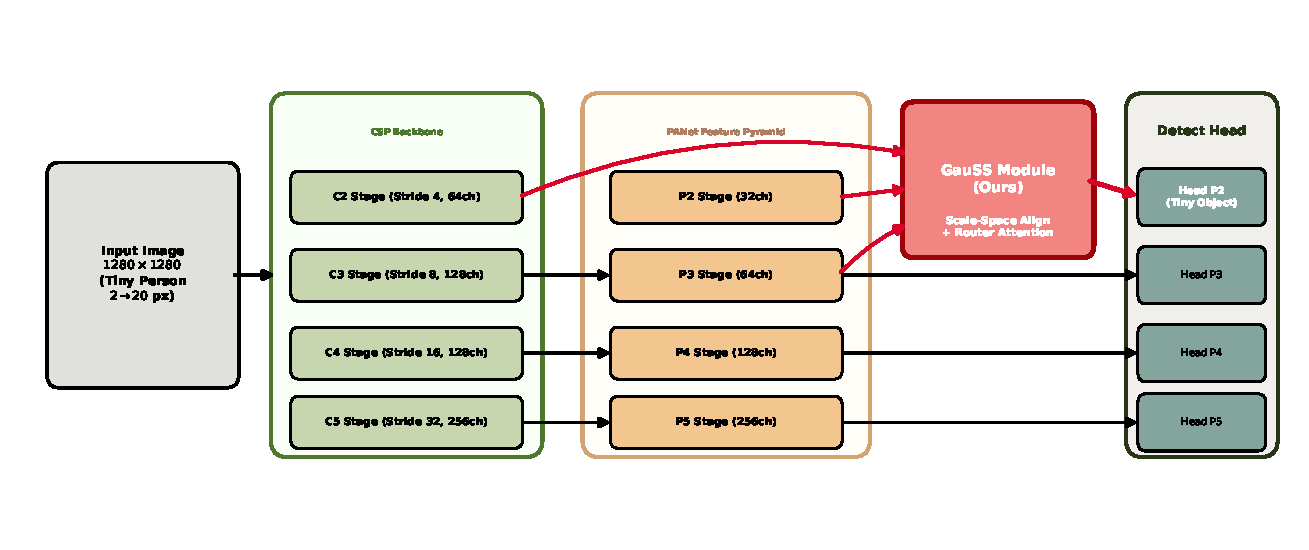
\includegraphics[width=\linewidth]{figures/11_overall_gauss_pipeline.pdf}
  \caption{\textbf{Overall Architecture of the YOLO26n-P2 + GauSS Detector}: GauSS operates at the junction between Backbone Layer 2 ($C_2$), the lateral neck ($P_3$), and contextual features ($P_4$), refining the stride-4 representation before passing to the detection head.}
  \label{fig:pipeline_overview}
\end{figure*}

\subsection{Architectural Overview}
\label{sec:arch_overview}
As shown in Figure~\ref{fig:pipeline_overview}, the detector adopts a single-stage anchor-free design with four detection strides: $P_2$ (stride 4), $P_3$ (stride 8), $P_4$ (stride 16), and $P_5$ (stride 32). An input image $\mathbf{I} \in \mathbb{R}^{3 \times H \times W}$ passes through a CSPDarknet backbone~\cite{bochkovskiy2020yolov4}, producing hierarchical feature maps $\mathbf{C}_2, \mathbf{C}_3, \mathbf{C}_4, \mathbf{C}_5$ at strides 4, 8, 16, and 32. Throughout this paper, $1\times1$ convolutions denote pointwise channel projections, and DWConv denotes depthwise convolution; both follow the depthwise-separable factorization popularized by MobileNets~\cite{howard2017mobilenets} and Xception~\cite{chollet2017xception}. Convolutional blocks are normalized with Batch Normalization (BN)~\cite{ioffe2015batch} and activated with SiLU~\cite{elfwing2018silu,ramachandran2017swish}, i.e., $\text{SiLU}(x) = x \cdot \sigma(x)$.

To provide spatial sampling for tiny objects, a stride-4 ($P2$) detection level is integrated. To prevent direct lateral concatenation from swamping target activations with sea clutter, GauSS is positioned at the intersection of $\mathbf{C}_2$, $\mathbf{P}_3$, and $\mathbf{P}_4$ (Figure~\ref{fig:gauss_router}). Table~\ref{tab:notations} details tensor dimensions and notations.

\begin{table*}[t]
\centering
\footnotesize
\caption{\textbf{Notation, Module Definitions, and Tensor Dimensions across the GauSS Pipeline}. Spatial shapes assume an input image of size $1280 \times 1280$ pixels.}
\label{tab:notations}
\begin{tabularx}{\textwidth}{lXl}
\toprule
\textbf{Symbol} & \textbf{Description} & \textbf{Dimension / Shape} \\
\midrule
$\mathbf{C}_2, \mathbf{P}_3, \mathbf{P}_4$ & Multi-scale input features (backbone stride 4, neck stride 8, context stride 16) & $\mathbb{R}^{64 \times 320 \times 320}, \mathbb{R}^{64 \times 160 \times 160}, \mathbb{R}^{128 \times 80 \times 80}$ \\
$\mathbf{S}_2, \mathbf{S}_3, \mathbf{S}_4$ & Channel-projected features ($1\times 1$ conv to unified hidden dimension $d=32$) & $\mathbb{R}^{32 \times 320 \times 320}, \mathbb{R}^{32 \times 160 \times 160}, \mathbb{R}^{32 \times 80 \times 80}$ \\
$\mathbf{X}_0$ & Fused base stride-4 feature: $\text{SiLU}(\text{BN}(\mathbf{S}_2 + \text{Interp}(\mathbf{S}_3)))$ & $\mathbb{R}^{32 \times 320 \times 320}$ \\
$\mathbf{L}_1, \mathbf{L}_2$ & Gaussian filtered features across scale regimes $\sigma_1 \in [0.4, 0.9], \sigma_2 \in [1.1, 1.8]$ & $\mathbb{R}^{32 \times 320 \times 320}$ \\
$\mathbf{B}_{\text{high}}, \mathbf{B}_{\text{mid}}, \mathbf{B}_{\text{low}}$ & Decomposed scale-space frequency bands: $\mathbf{X}_0 - \mathbf{L}_1, \; \mathbf{L}_1 - \mathbf{L}_2, \; \mathbf{L}_2$ & $\mathbb{R}^{32 \times 320 \times 320}$ \\
$\mathbf{R}_{\text{high}}, \mathbf{R}_{\text{mid}}, \mathbf{R}_{\text{low}}$ & Refined sub-pixel band representations ($\text{PixelUnshuffle}(2) + \text{DWConv}$) & $\mathbb{R}^{32 \times 160 \times 160}$ \\
$\mathbf{C}_{\text{ctx}}$ & Multi-scale dilated context guidance from $\mathbf{S}_3, \mathbf{S}_4$ ($r \in \{1, 2, 3\} + \text{Softmax Gate}$) & $\mathbb{R}^{32 \times 160 \times 160}$ \\
$\mathbf{Z}$ & Spatial routing logits computed via depthwise $3\times 3$ and $1\times 1$ conv on $\mathbf{U}$ & $\mathbb{R}^{4 \times 160 \times 160}$ \\
$\mathbf{a}_{\text{bands}}, m_{\text{gate}}$ & Dynamic routing weights: $\mathbf{a}_{\text{bands}} = \text{Softmax}(\mathbf{Z}_{1:3})$, $m_{\text{gate}} = \text{Sigmoid}(\mathbf{Z}_4)$ & $\mathbb{R}^{3 \times 160 \times 160}, \mathbb{R}^{1 \times 160 \times 160}$ \\
$\mathbf{F}_{\text{band}}$ & Synthesized band feature: $a_h \mathbf{R}_{\text{high}} + a_m \mathbf{R}_{\text{mid}} + a_l \mathbf{R}_{\text{low}} + \gamma_h \mathbf{R}_{\text{high}}$ & $\mathbb{R}^{32 \times 160 \times 160}$ \\
$\mathbf{R}_{\text{low}}^{\text{att}}$ & Saliency-attenuated low-band context: $\mathbf{R}_{\text{low}} \odot (1.0 - 0.5 \cdot \mathbf{M}_{\text{sal}})$ & $\mathbb{R}^{32 \times 160 \times 160}$ \\
$\mathbf{F}_{\text{route}}$ & Mixed feature from detail ($3\times 3$) and structural ($5\times 5$) branches & $\mathbb{R}^{32 \times 160 \times 160}$ \\
$\mathbf{P}_2^{\text{aligned}}$ & Final aligned Stride-4 output feature to detection head & $\mathbb{R}^{32 \times 320 \times 320}$ \\
\bottomrule
\end{tabularx}
\end{table*}

\begin{figure*}[t]
  \centering
  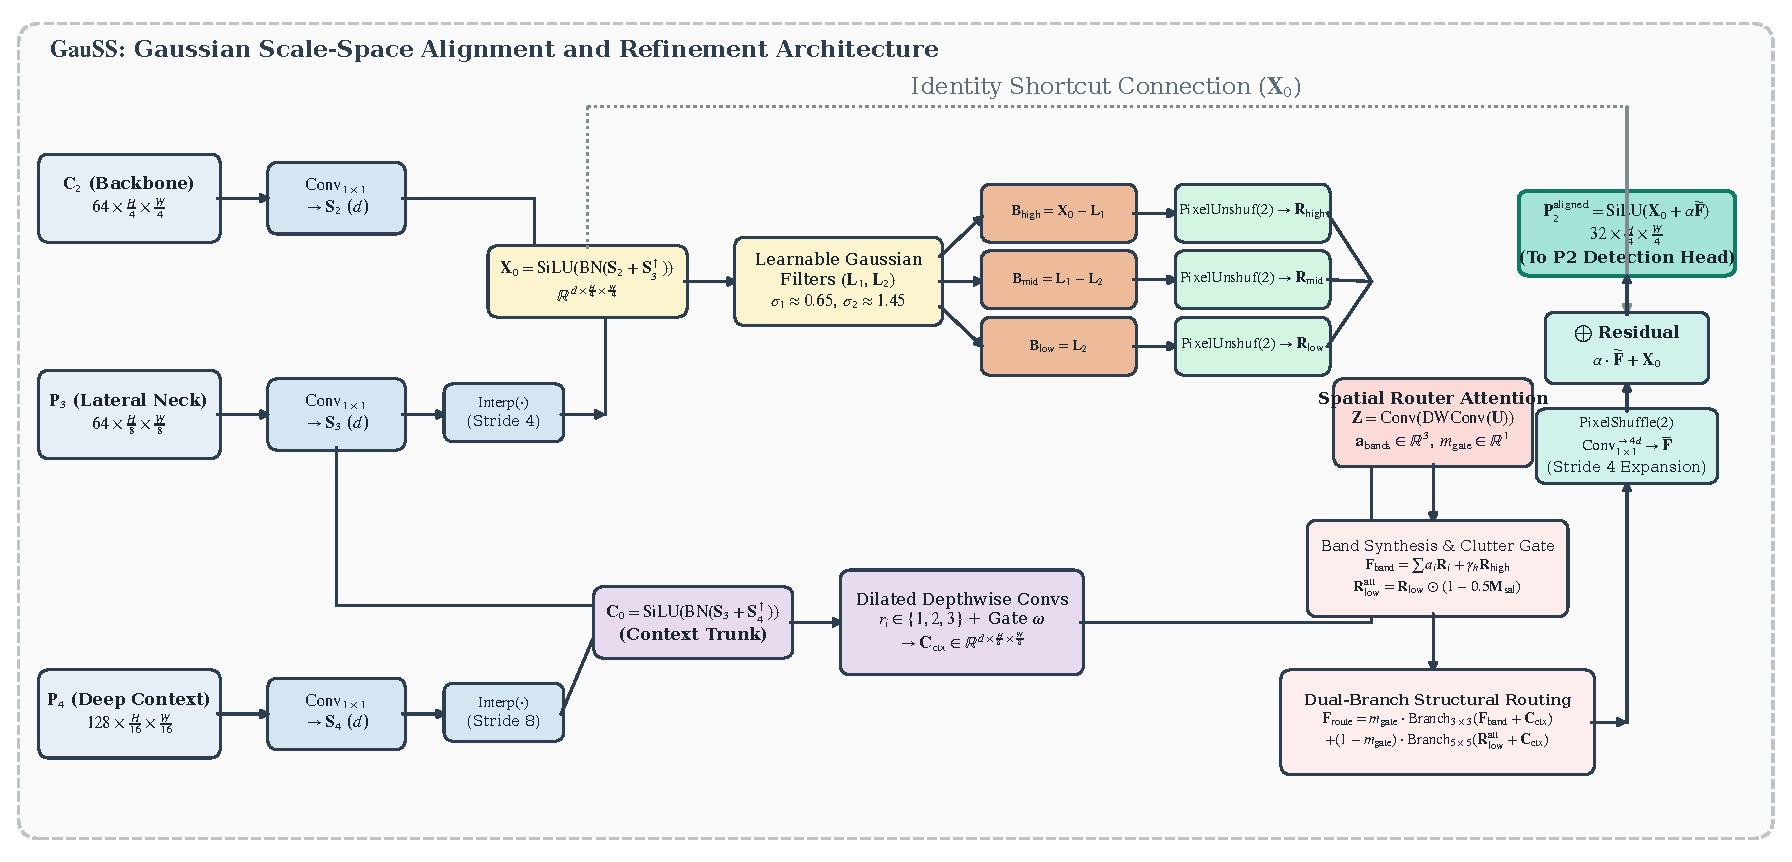
\includegraphics[width=\linewidth]{figures/10_gauss_router_architecture.pdf}
  \caption{\textbf{Detailed Architectural Diagram of the GauSS Module}: Multi-scale decomposition via separable Gaussian filtering on base feature $\mathbf{X}_0$, multi-scale dilated context aggregation, dense spatial routing, dual-path synthesis, and stride-4 residual reconstruction.}
  \label{fig:gauss_router}
\end{figure*}

\subsection{Discrete Gaussian Scale-Space Formulation}
\label{sec:scalespace_formulation}
Axiomatic scale-space theory~\cite{witkin1983scale,koenderink1984structure,lindeberg1994scale} establishes that multi-scale representation without spurious extrema generation is uniquely governed by parameterized continuous Gaussian diffusion:
\begin{equation}
  L(\mathbf{x}; \sigma) = g(\mathbf{x}; \sigma) * f(\mathbf{x}),
  \label{eq:scalespace_continuous}
\end{equation}
\begin{equation}
  g(\mathbf{x}; \sigma) = \frac{1}{2\pi\sigma^2} \exp\left( -\frac{\|\mathbf{x}\|^2}{2\sigma^2} \right),
  \label{eq:gaussian_kernel_def}
\end{equation}
where $\mathbf{x} \in \mathbb{R}^2$ denotes spatial coordinates and $*$ denotes convolution. To embed this principle inside feature pyramids, GauSS takes multi-scale inputs: $\mathbf{C}_2 \in \mathbb{R}^{64 \times \frac{H}{4} \times \frac{W}{4}}$, $\mathbf{P}_3 \in \mathbb{R}^{64 \times \frac{H}{8} \times \frac{W}{8}}$, and $\mathbf{P}_4 \in \mathbb{R}^{128 \times \frac{H}{16} \times \frac{W}{16}}$. Inputs are projected to a unified hidden dimension $d = 32$:
\begin{equation}
  \mathbf{S}_2 = \text{Conv}_{1\times 1}(\mathbf{C}_2), \quad \mathbf{S}_3 = \text{Conv}_{1\times 1}(\mathbf{P}_3),
  \label{eq:proj_s23}
\end{equation}
\begin{equation}
  \mathbf{S}_4 = \text{Conv}_{1\times 1}(\mathbf{P}_4),
  \label{eq:proj_s4}
\end{equation}
\begin{equation}
  \mathbf{X}_0 = \text{SiLU}\big( \text{BN}(\mathbf{S}_2 + \text{Interp}(\mathbf{S}_3)) \big),
  \label{eq:proj_x0}
\end{equation}
where $\text{Interp}(\cdot)$ denotes nearest-neighbor upsampling to stride 4.

On fused representation $\mathbf{X}_0 \in \mathbb{R}^{d \times \frac{H}{4} \times \frac{W}{4}}$, GauSS applies a \textit{Learnable Separable Gaussian Filter} across two scale regimes per channel:
\begin{equation}
  \mathbf{L}_k = g_y(\sigma_{k,y}) * \left( g_x(\sigma_{k,x}) * \text{Pad}(\mathbf{X}_0) \right), \quad k \in \{1, 2\},
  \label{eq:gaussian_filter}
\end{equation}
where $\sigma_{k,x}, \sigma_{k,y}$ are channel-wise learnable parameters bounded via sigmoid transforms: $\sigma_1 \in [0.4, 0.9]$ (radius $r_1=2$, support $5\times 5$, initialized at $0.65$) and $\sigma_2 \in [1.1, 1.8]$ (radius $r_2=4$, support $9\times 9$, initialized at $1.45$). Note that because filtering operates on the stride-4 grid ($1\text{ cell} = 4\text{ image pixels}$), the physical scale support corresponds to $\sigma_{1,\text{img}} \approx 2.6\text{ px}$ and $\sigma_{2,\text{img}} \approx 5.8\text{ px}$. 1D discrete kernels are constructed by softmax normalization over integer grid offsets:
\begin{equation}
  g(u; \sigma) = \text{Softmax}\left( -\frac{u^2}{2\sigma^2} \right), \quad u \in \{-r_k, \dots, r_k\}.
  \label{eq:kernel_construction}
\end{equation}
From discrete Gaussian representations $(\mathbf{X}_0, \mathbf{L}_1, \mathbf{L}_2)$, GauSS decomposes features into three complementary frequency bands:
\begin{equation}
  \mathbf{B}_{\text{high}} = \mathbf{X}_0 - \mathbf{L}_1,
  \label{eq:band_h}
\end{equation}
\begin{equation}
  \mathbf{B}_{\text{mid}} = \mathbf{L}_1 - \mathbf{L}_2,
  \label{eq:band_m}
\end{equation}
\begin{equation}
  \mathbf{B}_{\text{low}} = \mathbf{L}_2.
  \label{eq:band_l}
\end{equation}
Here, $\mathbf{B}_{\text{high}}$ captures high-frequency edge and contour details, $\mathbf{B}_{\text{mid}}$ responds to band-pass structural morphology ($8\text{--}12\text{ px}$ targets), and $\mathbf{B}_{\text{low}}$ provides low-pass macroscopic context.
Each band is refined through a lightweight sub-pixel encoder branch comprising $\text{PixelUnshuffle}(2)$, depthwise separable convolutions, and residual addition. $\text{PixelUnshuffle}(2)$ is the exact inverse of the sub-pixel rearrangement operator $\text{PixelShuffle}(2)$ introduced for efficient super-resolution by Shi~\etal~\cite{shi2016pixelshuffle}: it reorganizes the $H/4 \times W/4$ grid to $H/8 \times W/8$ and quadruples the channels, which a $1\times 1$ conv projects back to $d$, yielding $\{\mathbf{R}_{\text{high}}, \mathbf{R}_{\text{mid}}, \mathbf{R}_{\text{low}}\} \in \mathbb{R}^{d \times \frac{H}{8} \times \frac{W}{8}}$.

\subsection{Multi-Scale Context Gating and Spatial Routing}
\label{sec:router_attention}
To guide scale-space bands with deep semantic context without blurring tiny instances, deeper features are fused: $\mathbf{C}_0 = \text{SiLU}(\text{BN}(\mathbf{S}_3 + \text{Interp}(\mathbf{S}_4)))$. Three parallel dilated depthwise $3\times 3$ convolutions with dilation rates $r_i \in \{1, 2, 3\}$ capture multi-scale receptive fields:
\begin{equation}
  \mathbf{T}_i = \text{SiLU}\big(\text{BN}(\text{DWConv}_{r_i}(\mathbf{C}_0))\big).
  \label{eq:dilated_context}
\end{equation}
A channel softmax gate $\boldsymbol{\omega} = \text{Softmax}(\text{Conv}_{1\times 1}(\mathbf{C}_0)) \in \mathbb{R}^3$ modulates the contributions of the dilated branches:
\begin{equation}
  \mathbf{C}_{\text{ctx}} = \text{SiLU}\left(\mathbf{C}_0 + \sum_{i=1}^3 \omega_i \mathbf{T}_i\right).
  \label{eq:context_fusion}
\end{equation}
A lightweight spatial router then computes per-location band-selection logits. Its four output channels are split into three band logits $\mathbf{a}_{\text{bands}} = (a_h, a_m, a_l)$ and one mixing logit $m_{\text{gate}}$:
\begin{equation}
  \mathbf{U} = \text{SiLU}(\mathbf{R}_{\text{high}} + \mathbf{R}_{\text{mid}} + \mathbf{R}_{\text{low}} + \mathbf{C}_{\text{ctx}}),
  \label{eq:routing_u}
\end{equation}
\begin{equation}
  \mathbf{Z} = \text{Conv}_{1\times 1}\big(\text{SiLU}(\text{BN}(\text{DWConv}_{3\times 3}(\mathbf{U})))\big),
  \label{eq:routing_logits}
\end{equation}
\begin{equation}
  \mathbf{a}_{\text{bands}} = \text{Softmax}(\mathbf{Z}_{1:3}), \quad m_{\text{gate}} = \text{Sigmoid}(\mathbf{Z}_4),
  \label{eq:routing_gate}
\end{equation}
where $\mathbf{Z} \in \mathbb{R}^{4 \times \frac{H}{8} \times \frac{W}{8}}$. $\mathbf{a}_{\text{bands}}$ provides spatial routing weights, while $m_{\text{gate}}$ balances detail and structural paths.

Adaptive band synthesis is anchored with a high-band direct shortcut:
\begin{equation}
  \mathbf{F}_{\text{band}} = a_h \mathbf{R}_{\text{high}} + a_m \mathbf{R}_{\text{mid}} + a_l \mathbf{R}_{\text{low}} + \gamma_h \mathbf{R}_{\text{high}},
  \label{eq:band_synthesis}
\end{equation}
where $\gamma_h = 0.5 \cdot \text{Sigmoid}(\gamma_{h,\text{raw}})$ bounds the high-band shortcut to $(0, 0.5)$, retaining sub-8\,px gradient energy. Background wave clutter is attenuated via a learned saliency gate on the low-band branch:
\begin{equation}
  \mathbf{M}_{\text{sal}} = \text{Sigmoid}\big(\text{Conv}_{1\times 1}(\mathbf{C}_{\text{ctx}})\big),
  \label{eq:saliency_mask}
\end{equation}
\begin{equation}
  \mathbf{R}_{\text{low}}^{\text{att}} = \mathbf{R}_{\text{low}} \odot (1.0 - 0.5 \cdot \mathbf{M}_{\text{sal}}).
  \label{eq:saliency_att}
\end{equation}
Detail ($3\times 3$) and structural ($5\times 5$) paths are then mixed:
\begin{align}
  \mathbf{F}_{\text{route}} &= m_{\text{gate}} \cdot \text{Branch}_{3\times 3}(\mathbf{F}_{\text{band}} + \mathbf{C}_{\text{ctx}}) \nonumber \\
  &\quad + (1 - m_{\text{gate}}) \cdot \text{Branch}_{5\times 5}(\mathbf{R}_{\text{low}}^{\text{att}} + \mathbf{C}_{\text{ctx}}).
  \label{eq:f_route}
\end{align}
Finally, features are reconstructed to stride 4. A $1\times 1$ conv expands $\mathbf{F}_{\text{route}}$ to $4d$ channels, and $\text{PixelShuffle}(2)$~\cite{shi2016pixelshuffle} returns them to $d$ channels at stride 4. With bounded gain $\alpha = 0.5 \cdot \text{Sigmoid}(a_\alpha)$ and refined residual $\widetilde{\mathbf{F}}$, the aligned feature is formed:
\begin{equation}
  \widetilde{\mathbf{F}} = \text{PixelShuffle}(2)\big(\text{BN}(\text{Conv}_{1\times 1}^{\to 4d}(\mathbf{F}_{\text{route}}))\big),
  \label{eq:f_tilde}
\end{equation}
\begin{equation}
  \mathbf{P}_2^{\text{aligned}} = \text{SiLU}\big( \mathbf{X}_0 + \alpha \cdot \widetilde{\mathbf{F}} \big).
  \label{eq:p2_aligned}
\end{equation}

\subsection{Parameter Breakdown}
\label{sec:param_breakdown}
Table~\ref{tab:param_breakdown} provides a detailed parameter decomposition of the GauSS module. The entire module contains exactly $34{,}666$ trainable parameters ($+1.38\%$ overhead on the $2{,}516{,}240$ parameter baseline), embedding multi-scale filtering and routing with minimal memory burden.

\begin{table}[t]
\centering
\footnotesize
\caption{\textbf{Exact Trainable Parameter Breakdown of GauSS} ($d=32$). Total module parameters: $34{,}666$ weights.}
\label{tab:param_breakdown}
\begin{tabularx}{\linewidth}{lXr}
\toprule
\textbf{Submodule} & \textbf{Component Layers / Tensors} & \textbf{Params} \\
\midrule
Channel Projections & $\text{Conv}_{1\times 1}$ on $C_2, P_3, P_4$ ($8{,}192$) + BN2 ($64$) & 8,256 \\
Gaussian Filtering & Learnable 1D parameters ($\sigma_{1x,1y}, \sigma_{2x,2y}$) & 128 \\
Band Encoders & 3 branches ($\text{PixelUnshuffle} + \text{DW} + \text{PW} + \text{BN}$) & 16,800 \\
Dilated Context & 3 DWConv branches ($r \in \{1,2,3\}$) + Gate ($99$) & 1,155 \\
Saliency Gating & Low-band attention $1\times 1$ conv ($32 \times 1 + 1$) & 33 \\
Spatial Router & Depthwise $3\times 3$ ($288$) + BN ($64$) + Conv ($132$) & 484 \\
Dual Refinement & $3\times 3$ detail ($1{,}440$) + $5\times 5$ structural ($1{,}952$) & 3,392 \\
Reconstruction & Conv $1\times 1$ $\to 4d$ ($4{,}096$) + BN ($256$) & 4,352 \\
Gain Scalars & Learnable scalars ($\alpha_{\text{raw}}$, $\gamma_{h,\text{raw}}$) & 2 \\
\midrule
\textbf{Total GauSS Overhead} & & \textbf{34,666} \\
\bottomrule
\end{tabularx}
\end{table}

\subsection{Head Formulation and Regression Loss}
\label{sec:loss_head}
Anchor-free detectors historically used Generalized Focal Loss (GFL)~\cite{li2020gfl,li2021gflv2} with Distribution Focal Loss ($\text{DFL}$) across 16 discrete bins to model box boundary uncertainty. However, for ultra-tiny objects ($2\text{--}8\text{ px}$), multi-bin distribution modeling introduces spatial variance. In our architecture, following YOLO26's native end-to-end regression design~\cite{ultralytics2026yolo}, bounding box regression is parametrized with $\text{reg\_max} = 1$, collapsing coordinate offsets into deterministic scalars ($\mathcal{L}_{\text{DFL}} = 0$). Training utilizes the Task-Aligned One-Stage Object Detection (TOOD)~\cite{feng2021tood} objective with CIoU~\cite{zheng2020diou} loss -- a strict-IoU metric family that also motivates GIoU~\cite{rezatofighi2019giou} and NWD~\cite{wang2021nwd} for tiny boxes -- and auxiliary $\ell_1$ regression:
\begin{equation}
  \mathcal{L}_{\text{total}} = \lambda_{\text{cls}} \mathcal{L}_{\text{cls}} + \lambda_{\text{box}} \mathcal{L}_{\text{CIoU}} + \lambda_{\ell_1} \mathcal{L}_{\ell_1},
  \label{eq:total_loss}
\end{equation}
where $\lambda_{\text{cls}} = 0.5, \lambda_{\text{box}} = 7.5, \lambda_{\ell_1} = 1.0$. Crucially, both the baseline and GauSS share this exact regression formulation and use identical post-processing.

\section{Experimental Setup}
\label{sec:setup}

\subsection{Datasets and Evaluation Protocols}
\textbf{TinyPerson (WACV 2020)}~\cite{yu2020tinyperson}: The dataset contains high-resolution maritime and coastal images. Standard annotations provide 1,610 frames sampled at 50-frame intervals from video sequences. The benchmark partitions these into 746 training frames and 786 evaluation frames across 31 distinct video sequences, preventing frame-level bleed between splits. Ground truth includes 13,687 positive person boxes, 1,989 ignore boxes, and 2,832 uncertain boxes. Following the official benchmark, instances are categorized by absolute scale $s = \sqrt{w \cdot h}$ (in pixels):
\begin{itemize}
    \item $tiny1$: $s \in [2, 8)$ px (2,333 ground-truth instances).
    \item $tiny2$: $s \in [8, 12)$ px (2,778 ground-truth instances).
    \item $tiny3$: $s \in [12, 20]$ px (3,767 ground-truth instances).
    \item $tiny$: $s \in [2, 20]$ px (8,878 ground-truth instances).
    \item $small$: $s \in (20, 32]$ px (2,485 ground-truth instances).
    \item $reasonable$: $s \in (32, \infty)$ px (2,324 ground-truth instances).
    \item $all$: $s \in [2, \infty)$ px (13,687 ground-truth instances).
\end{itemize}

\textbf{VisDrone-DET (TPAMI Standard)}~\cite{zhu2021visdrone}: Contains 10 categories captured from UAVs (548 validation images and 1,610 test-dev images).

\subsection{Standardized Inference Protocol}
Evaluation on TinyPerson adheres strictly to the official TOV benchmarking protocol:
\begin{enumerate}
    \item High-resolution images are sliced into tiles of $640 \times 512$ pixels with horizontal and vertical overlaps of $100$ pixels (averaging $23.4$ tiles per image).
    \item Sub-image predictions are mapped back to full image coordinates.
    \item Global NMS merges candidate boxes with an IoU threshold of $0.50$ (greedy non-maximum suppression~\cite{neubeck2006nms,ren2015faster}; greedy threshold-based suppression is the failure mode that Soft-NMS~\cite{bodla2017softnms} was designed to soften), pre-NMS top-$2000$ proposals, and max $1000$ detections per image. Normal targets are matched by IoU~\cite{rezatofighi2019giou,zheng2020diou}; ignore and uncertain regions use Intersection-over-Detection ($\text{IoD} > 0.50$) to avoid penalizing valid detections inside dense crowd regions.
\end{enumerate}

\subsection{Training Hyperparameters}
Both Baseline (YOLO26n-P2) and GauSS are trained from scratch without external pre-training: $150$ epochs, input resolution $1280 \times 1280$, batch size $8$, AdamW optimizer~\cite{loshchilov2017adamw} ($\text{lr}_0 = 0.002, \text{lrf} = 0.1$, cosine schedule~\cite{loshchilov2016sgdr}), 5-epoch warmup, and FP16 mixed precision. Training uses only the 746 training frames; no hyperparameters were tuned on the 786 test frames.

\begin{figure*}[t]
  \centering
  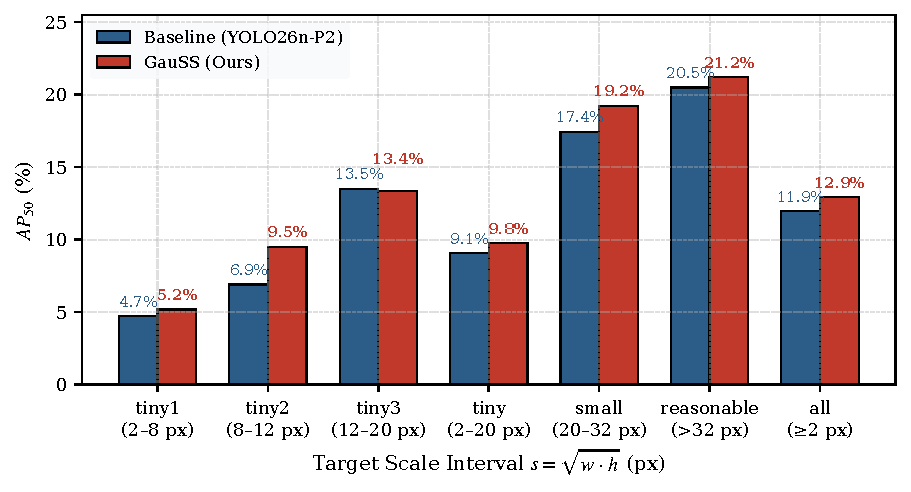
\includegraphics[width=\linewidth]{figures/01_tinyperson_ap50_by_size.pdf}
  \caption{\textbf{Fine-grained Size-Bin Performance on TinyPerson (150 Epochs)}: Evaluating $AP_{50}$ across standard academic bins: $tiny1$ ($2\text{--}8\text{ px}$), $tiny2$ ($8\text{--}12\text{ px}$), $tiny3$ ($12\text{--}20\text{ px}$), $tiny$ ($2\text{--}20\text{ px}$), $small$ ($20\text{--}32\text{ px}$), $reasonable$ ($>32\text{ px}$), and $all$ ($\ge 2\text{ px}$). GauSS achieves $+2.59\text{ pp}$ improvement on $tiny2$ and $+0.98\text{ pp}$ overall.}
  \label{fig:size_bin_ap}
\end{figure*}

\section{Results and Analysis}
\label{sec:results}

\begin{table*}[t]
\centering
\footnotesize
\setlength{\tabcolsep}{4.5pt}
\caption{\textbf{Comprehensive Experimental Comparison on TinyPerson Test Set (786 Images, 13,687 Targets) across 50 and 150 Epochs}. Evaluated under standardized tiled slicing ($640 \times 512$, overlap $100$). GT denotes the exact ground-truth instance count in each scale bracket. Differences ($\Delta$) are absolute percentage points (pp). Bold highlights the superior 150-epoch model.}
\label{tab:main_tinyperson}
\begin{tabular*}{\textwidth}{@{\extracolsep{\fill}}lcccccc@{}}
\toprule
\textbf{Metric / Scale Bracket} & \textbf{GT Boxes} & \textbf{Base (50e)} & \textbf{Base (150e)} & \textbf{GauSS (50e)} & \textbf{GauSS (150e)} & \textbf{$\Delta$ (vs. Base 150e)} \\
\midrule
$AP_{50}^{\text{all}}$ ($\ge 2$ px)     & 13,687 & 10.02 & 11.95 & 10.91 & \textbf{12.94} & \textbf{+0.98} pp \\
$AP_{50}^{\text{tiny}}$ ($2\text{--}20$ px)  & 8,878  & 7.06  & 9.07  & 8.37  & \textbf{9.76}  & \textbf{+0.69} pp \\
$AP_{50}^{\text{tiny1}}$ ($2\text{--}8$ px)   & 2,333  & 3.20  & 4.72  & 4.43  & \textbf{5.18}  & \textbf{+0.46} pp \\
$AP_{50}^{\text{tiny2}}$ ($8\text{--}12$ px)  & 2,778  & 5.96  & 6.90  & 7.04  & \textbf{9.50}  & \textbf{+2.59} pp \\
$AP_{50}^{\text{tiny3}}$ ($12\text{--}20$ px) & 3,767  & 10.84 & 13.51 & 11.92 & 13.37          & $-$0.14 pp \\
$AP_{50}^{\text{small}}$ ($20\text{--}32$ px) & 2,485  & 15.51 & 17.43 & 16.79 & \textbf{19.23} & \textbf{+1.80} pp \\
$AP_{50}^{\text{reasonable}}$ ($>32$ px)      & 2,324  & 17.67 & 20.49 & 16.52 & \textbf{21.20} & \textbf{+0.72} pp \\
\midrule
$AP_{25}^{\text{all}}$ (IoU 0.25)        & 13,687 & 17.52 & 21.28 & 19.82 & 20.68          & $-$0.61 pp \\
$AP_{75}^{\text{all}}$ (IoU 0.75)        & 13,687 & 0.60  & 1.28  & 1.43  & \textbf{1.40}  & \textbf{+0.11} pp \\
Mean $AP_{25,50,75}^{\text{all}}$        & 13,687 & 9.38  & 11.51 & 10.72 & \textbf{11.67} & \textbf{+0.16} pp \\
\midrule
$MR_{50}^{\text{all}}$ (miss rate, $\downarrow$)  & 13,687 & 97.49 & 96.93 & 97.43 & \textbf{96.73} & \textbf{$-$0.21} pp \\
$MR_{50}^{\text{tiny}}$ ($\downarrow$)           & 8,878  & 97.40 & 95.90 & 96.57 & \textbf{95.87} & \textbf{$-$0.03} pp \\
$MR_{50}^{\text{tiny1}}$ ($\downarrow$)          & 2,333  & 97.26 & 95.83 & 96.34 & 96.01          & $+$0.18 pp \\
$MR_{50}^{\text{tiny2}}$ ($\downarrow$)          & 2,778  & 96.65 & 95.10 & 95.42 & \textbf{93.52} & \textbf{$-$1.58} pp \\
$MR_{50}^{\text{tiny3}}$ ($\downarrow$)          & 3,767  & 94.39 & 92.11 & 92.65 & 92.57          & $+$0.46 pp \\
$MR_{50}^{\text{small}}$ ($\downarrow$)          & 2,485  & 91.42 & 89.98 & 90.58 & \textbf{88.73} & \textbf{$-$1.26} pp \\
\bottomrule
\end{tabular*}
\end{table*}

\begin{figure*}[t]
  \centering
  \begin{minipage}{0.48\textwidth}
    \centering
    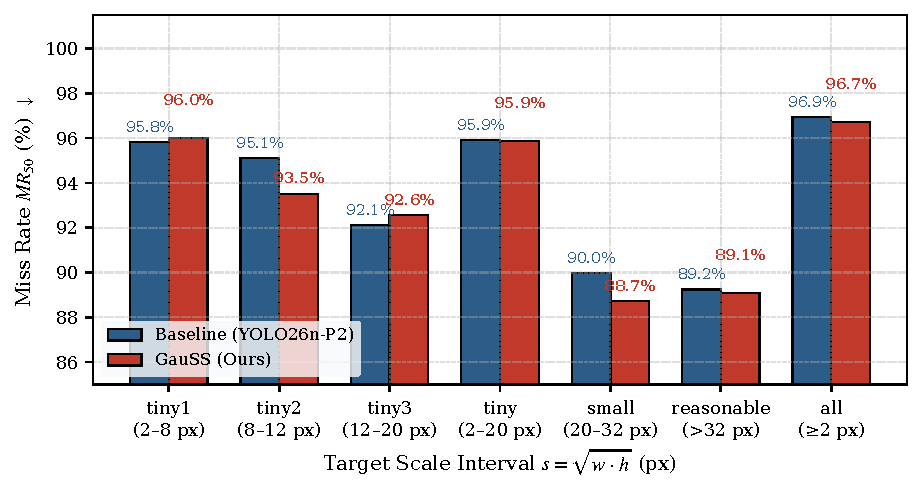
\includegraphics[width=\linewidth]{figures/02_tinyperson_miss_rate.pdf}
    \caption{\textbf{Miss Rate Analysis ($MR_{50}$)} across size-bins. GauSS reduces missed targets in $tiny2$ by $1.58\text{ pp}$ and in $small$ by $1.26\text{ pp}$. Minor fluctuations occur in $tiny1$ and $tiny3$.}
    \label{fig:miss_rate}
  \end{minipage}\hfill
  \begin{minipage}{0.48\textwidth}
    \centering
    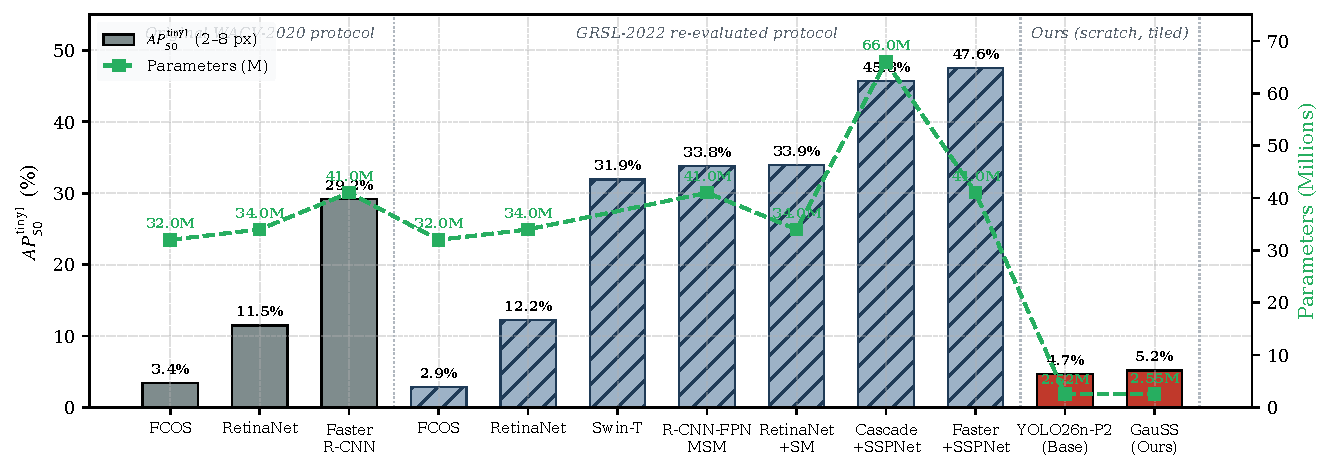
\includegraphics[width=\linewidth]{figures/03_international_tiny1_tradeoff.pdf}
    \caption{\textbf{TinyPerson $tiny1$ accuracy--parameter landscape}, grouped by evaluation protocol: \textbf{(a)} original benchmark numbers (WACV 2020); \textbf{(b)} two-stage zoo re-evaluated under a single GRSL 2022 protocol (hatched); \textbf{(c)} nano-scale detectors trained from scratch under our tiled protocol. Cross-protocol comparisons indicate context, not controlled comparisons; within group (a), GauSS reaches $5.18\%$ $tiny1$ AP versus $3.39\%$ for FCOS with $\sim$$12.5\times$ fewer parameters.}
    \label{fig:intl_tiny1}
  \end{minipage}
\end{figure*}

\subsection{Quantitative Performance and Scale-Bin Analysis}
Table~\ref{tab:main_tinyperson} and Figure~\ref{fig:size_bin_ap} report results across all scale intervals. At 150 epochs, GauSS achieves an overall $AP_{50}^{\text{all}}$ of $12.94\%$, an improvement of $+0.98\text{ pp}$ over the matched baseline ($11.95\%$).

\textbf{Scale-Bin Breakdown}:
\begin{itemize}
    \item \textit{$tiny2$ ($8\text{--}12$ px, 2,778 boxes)}: GauSS improves from $6.90\%$ to $9.50\%$ AP ($+2.59\text{ pp}$, $+37.5\%$ relative gain), and $MR_{50}^{\text{tiny2}}$ drops from $95.10\%$ to $93.52\%$ (Figure~\ref{fig:miss_rate}). The physical extent of objects in this bin ($8\text{--}12\text{ px}$) aligns closely with the effective receptive field of the learned scale parameters on stride 4 ($\sigma_{1,\text{img}} \approx 2.6\text{ px}, \sigma_{2,\text{img}} \approx 5.8\text{ px}$, supporting structures of $2\sigma \approx 5\text{--}12\text{ px}$). The band-pass signal $\mathbf{B}_{\text{mid}} = \mathbf{L}_1 - \mathbf{L}_2$ isolates these boundaries from low-frequency water gradients.
    \item \textit{$tiny1$ ($2\text{--}8$ px, 2,333 boxes)}: GauSS yields a moderate gain from $4.72\%$ to $5.18\%$ ($+0.46\text{ pp}$). Targets spanning fewer than 8 pixels occupy under $2 \times 2$ cells at stride 4 ($320 \times 320$), approaching the fundamental spatial Nyquist limit. The high-band residual path ($\gamma_h \mathbf{R}_{\text{high}}$) preserves gradient flow, but absolute performance remains constrained.
    \item \textit{$tiny3$ ($12\text{--}20$ px, 3,767 boxes)}: The baseline reaches $13.51\%$ while GauSS achieves $13.37\%$ ($-0.14\text{ pp}$). Targets above 12 pixels are already well captured by the lateral $P3$ stride-8 path, rendering stride-4 sub-pixel refinement less impactful.
    \item \textit{$small$ and $reasonable$ ($>20$ px, 4,809 boxes)}: GauSS improves $AP_{50}^{\text{small}}$ by $+1.80\text{ pp}$ ($19.23\%$ vs. $17.43\%$) and $reasonable$ by $+0.72\text{ pp}$ ($21.20\%$ vs. $20.49\%$).
\end{itemize}

\subsection{Cross-Epoch Stability and Variance Analysis}
As noted in Table~\ref{tab:main_tinyperson}, comparing models across 50 and 150 epochs reveals notable training dynamics. At 50 epochs, the largest gain appears in $tiny1$ ($+1.23\text{ pp}$), whereas at 150 epochs, optimization stabilizes around $tiny2$ ($+2.59\text{ pp}$), while $tiny1$ delta moderates to $+0.46\text{ pp}$. The $reasonable$ bin shifts from $-1.15\text{ pp}$ at 50e to $+0.72\text{ pp}$ at 150e. Because deep detectors trained from scratch on extreme aerial imagery exhibit run-to-run stochasticity, these cross-epoch variations underscore the necessity of multi-seed evaluations to establish confidence intervals.

\subsection{Comparative Reference on TinyPerson Benchmarks}
Table~\ref{tab:intl_comparison} and Figure~\ref{fig:intl_tiny1} place GauSS alongside published TinyPerson results, grouped by evaluation protocol. Because crop-rescaling schedules, training resolutions, augmentations, and evaluation rules differ substantially across studies, we quote each number from its original publication and mark the protocol family; cross-protocol comparison indicates context rather than a controlled ablation.

\textbf{(a) Original TinyPerson benchmark (WACV 2020)}: Faster R-CNN~\cite{ren2015faster}, RetinaNet~\cite{lin2017focal}, and FCOS~\cite{tian2019fcos} with ImageNet~\cite{deng2009imagenet,russakovsky2015imagenet}-pretrained ResNet-50 backbones ($>32\text{--}41\text{M}$ parameters) reach $43.55\%$, $30.82\%$, and $16.90\%$ $AP_{50}^{\text{tiny}}$, respectively, with crop-rescaling schedules~\cite{yu2020tinyperson}. GauSS, trained entirely from scratch with $2.55\text{M}$ parameters, attains $9.76\%$ $AP_{50}^{\text{tiny}}$ and $5.18\%$ on $tiny1$ -- above the FCOS ResNet-50 $tiny1$ reference ($3.39\%$) with $12.5\times$ fewer parameters.
\textbf{(b) Published TinyPerson results under two-stage pipelines (GRSL 2022)}: Hong~\etal~\cite{hong2022sspnet} re-evaluate a broad detector zoo under their preprocessing and report, among others, FCOS ($17.90\%$), RetinaNet~\cite{lin2017focal} ($33.53\%$), Faster R-CNN-FPN ($47.35\%$), Grid R-CNN~\cite{lu2019gridrcnn} ($47.14\%$), Libra R-CNN~\cite{pang2019librarcnn} ($44.68\%$), NAS-FPN~\cite{ghiasi2019nasfpn} ($37.75\%$), Swin-T~\cite{liu2021swin} ($40.52\%$), scale-matched variants~\cite{yu2020tinyperson,gong2021fusionfactor,jiang2021smplus} ($50.89\text{--}52.61\%$), Cascade R-CNN~\cite{cai2019cascade} ($57.19\%$), and their Faster R-CNN+SSPNet ($59.13\%$) on $AP_{50}^{\text{tiny}}$. The spread between identical detector names across protocol families (e.g., FCOS $16.90\%$ vs.~$17.90\%$; Faster R-CNN $43.55\%$ vs.~$57.05\%$ with PAFPN-style pipelines) quantifies how strongly protocol choices dominate absolute TinyPerson numbers.

\textbf{(c) Lightweight nano-scale regime ($<7\text{M}$ parameters)}: Chao~\etal~\cite{chao2025bpdyolo} report $39.1\%$ $mAP_{50}$ with the $1.50\text{M}$-parameter BPD-YOLO, alongside YOLOv8n+P2 ($38.0\%$, $2.93\text{M}$), YOLOv8n+P2+BiFPN ($38.4\%$, $2.34\text{M}$), and YOLOv8n+P2+AFPN ($39.2\%$, $6.05\text{M}$) on TinyPerson at input size $1024$ with Mosaic/MixUp augmentation, $300$-epoch schedules, the official $794$/$816$ split, and a single merged ``people'' class under the standard COCO $mAP_{50}$ protocol. These figures again use a different protocol family and are therefore not directly comparable to our tiled-protocol numbers; they establish that published nano-scale detectors operate in the same $38\text{--}39\%$ band under their settings.

\textbf{Why the absolute gap is large}: The $9.76\%$ vs.\ $38\text{--}59\%$ spread across groups is dominated by protocol choices rather than detector quality. Group (b) uses ImageNet-pretrained two-stage backbones trained on $640 \times 512$ cropped patches with the official per-class COCO-style AP; group (c) merges both person categories into one class and trains for $300$ epochs with strong augmentation. Our setting is deliberately harsher: training from scratch on $746$ frames with $150$ epochs and no Mosaic/MixUp. Additionally, our tiled evaluator scores detections class-agnostically against the pooled ground-truth set while retaining only the primary person category from the detector's two-class output, which suppresses absolute recall relative to both reference protocols. We therefore present Table~\ref{tab:intl_comparison} strictly as cross-protocol context; no cross-group delta should be read as a controlled comparison.

\begin{table}[t]
\centering
\scriptsize
\setlength{\tabcolsep}{2.5pt}
\caption{\textbf{Reference Comparison on TinyPerson Test Set}, grouped by protocol family. (a) Original benchmark numbers from Yu~\etal~\cite{yu2020tinyperson} (official per-class AP, ImageNet-pretrained). (b) Two-stage pipeline zoo from Hong~\etal~\cite{hong2022sspnet} (their re-implementation protocol). (c) Nano-scale YOLO family from Chao~\etal~\cite{chao2025bpdyolo} (input $1024$, Mosaic/MixUp, $300$ epochs, merged single class, COCO $mAP_{50}$). All prior entries are quoted verbatim from the cited publications; protocols, training schedules, and evaluation rules differ across groups, so cross-group deltas are indicative context only. YOLO26n-P2 and GauSS are trained from scratch without external pre-training under identical settings; see the text for the class-scoring difference that further separates our rows from all reference groups.}
\label{tab:intl_comparison}
\begin{tabular}{lcccc}
\toprule
\textbf{Model} & \textbf{Pretrain} & \textbf{Params} & \textbf{$AP_{50}^{\text{tiny}}$} & \textbf{$AP_{50}^{\text{tiny1}}$} \\
\midrule
\multicolumn{5}{l}{\textit{(a) Original benchmark~\cite{yu2020tinyperson}}}\\
Faster R-CNN~\cite{ren2015faster} & ImageNet & $\sim 41$M & 43.55\% & 29.21\% \\
RetinaNet~\cite{lin2017focal}    & ImageNet & $\sim 34$M & 30.82\% & 11.47\% \\
FCOS~\cite{tian2019fcos}         & ImageNet & $\sim 32$M & 16.90\% & 3.39\% \\
\midrule
\multicolumn{5}{l}{\textit{(b) Two-stage zoo~\cite{hong2022sspnet}}}\\
FCOS~\cite{tian2019fcos}                    & ImageNet & $\sim 32$M & 17.90\% & 2.88\% \\
RetinaNet~\cite{lin2017focal}               & ImageNet & $\sim 34$M & 33.53\% & 12.24\% \\
NAS-FPN~\cite{ghiasi2019nasfpn}             & ImageNet & --      & 37.75\% & 26.71\% \\
Swin-T~\cite{liu2021swin}                   & ImageNet & --      & 40.52\% & 31.92\% \\
Libra R-CNN~\cite{pang2019librarcnn}        & ImageNet & --      & 44.68\% & 27.08\% \\
Grid R-CNN~\cite{lu2019gridrcnn}            & ImageNet & --      & 47.14\% & 30.65\% \\
Faster R-CNN-FPN~\cite{lin2017fpn,ren2015faster} & ImageNet & $\sim 41$M & 47.35\% & 30.25\% \\
Faster R-CNN-FPN-MSM~\cite{yu2020tinyperson}     & ImageNet & $\sim 41$M & 50.89\% & 33.79\% \\
RetinaNet+SM~\cite{gong2021fusionfactor}    & ImageNet & $\sim 34$M & 52.56\% & 33.90\% \\
Faster R-CNN-FPN-MSM+~\cite{jiang2021smplus}& ImageNet & $\sim 41$M & 52.61\% & 34.20\% \\
Cascade R-CNN~\cite{cai2019cascade}         & ImageNet & $> 60$M & 57.19\% & 45.21\% \\
Faster R-CNN+SSPNet~\cite{hong2022sspnet}   & ImageNet & $> 41$M    & 59.13\% & 47.56\% \\
Cascade R-CNN+SSPNet~\cite{hong2022sspnet}  & ImageNet & $> 60$M    & 58.59\% & 45.75\% \\
\midrule
\multicolumn{5}{l}{\textit{(c) Nano-scale regime~\cite{chao2025bpdyolo} (1024px, Mosaic/MixUp, 300e, 1 class)}}\\
YOLOv8n+P2~\cite{chao2025bpdyolo}           & From scratch & 2.93M & 38.0\% & -- \\
YOLOv8n+P2+BiFPN~\cite{chao2025bpdyolo}     & From scratch & 2.34M & 38.4\% & -- \\
YOLOv8n+P2+AFPN~\cite{chao2025bpdyolo}      & From scratch & 6.05M & 39.2\% & -- \\
BPD-YOLO~\cite{chao2025bpdyolo}             & From scratch & 1.50M & 39.1\% & -- \\
\midrule
YOLO26n-P2 (Base)                    & None     & 2.52M          & 9.07\% & 4.72\% \\
\textbf{GauSS (Ours)}                & None     & \textbf{2.55M} & \textbf{9.76\%} & \textbf{5.18\%} \\
\bottomrule
\end{tabular}
\end{table}

\begin{figure*}[t]
  \centering
  \begin{minipage}{0.48\textwidth}
    \centering
    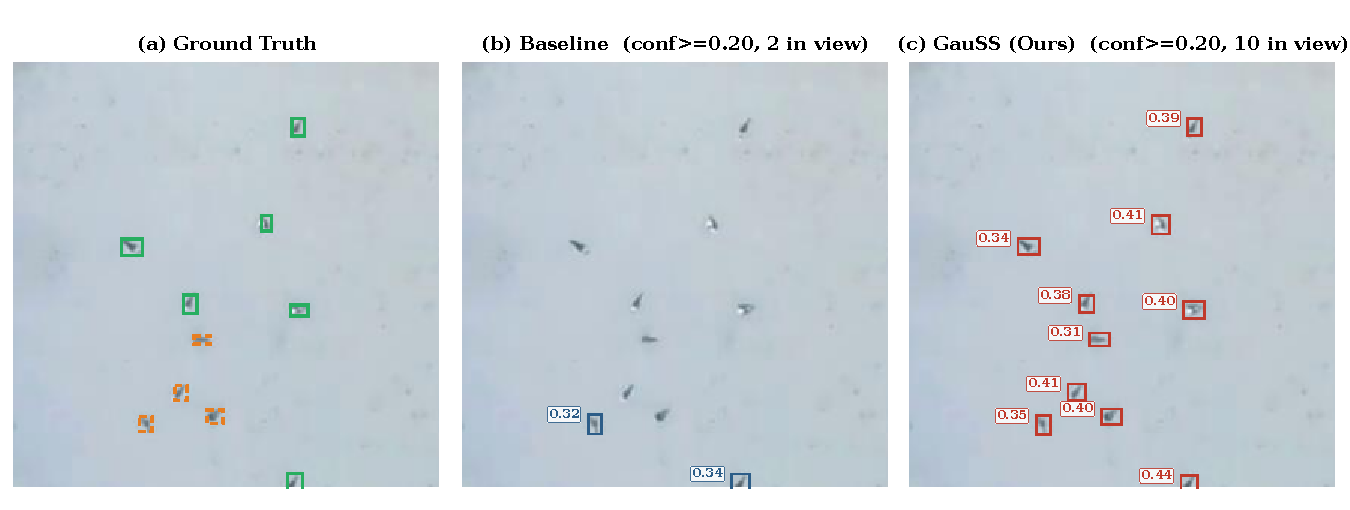
\includegraphics[width=\linewidth]{figures/12_qualitative_tiny_detections.pdf}
    \caption{\textbf{Qualitative Detection Comparison in an Offshore Swimmer Cluster}: Both models use the paper's tiled protocol ($640 \times 512$ tiles, overlap 100, global NMS IoU $0.50$) with an identical confidence threshold ($\ge 0.20$); every prediction above the threshold is drawn. In this $280 \times 280$~px zoom containing 6 tiny ground-truth swimmers, the baseline keeps 2 detections (conf. $0.32$--$0.34$) and GauSS keeps 10 (conf. $0.31$--$0.44$); frame-level totals are 12 vs.~21. Confidence scores are printed beside each box at source-image scale.}
    \label{fig:qualitative_detections}
  \end{minipage}\hfill
  \begin{minipage}{0.48\textwidth}
    \centering
    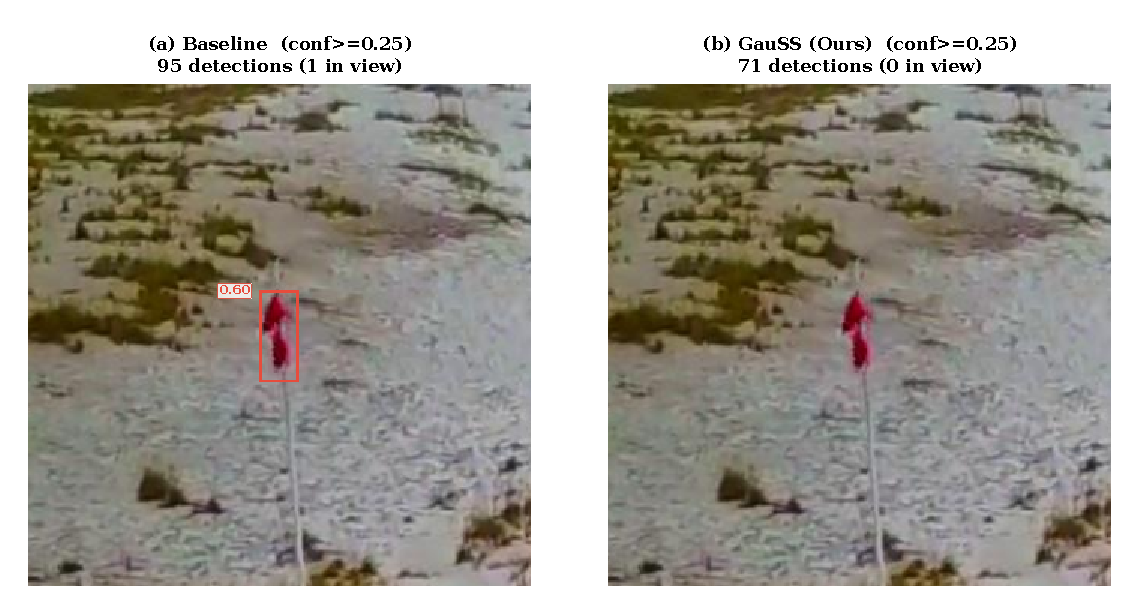
\includegraphics[width=\linewidth]{figures/13_sea_clutter_suppression.pdf}
    \caption{\textbf{False Alarm on a Wave Crest} (window with no ground-truth persons): Under the same tiled protocol with an identical threshold ($\ge 0.25$), the baseline fires one high-confidence false alarm ($0.60$) on reflective clutter, whereas GauSS reports no detection in this region. Frame-level totals drop from 95 to 71 detections; this is a qualitative example rather than an aggregate statistic.}
    \label{fig:sea_clutter}
  \end{minipage}
\end{figure*}

\begin{figure*}[t]
  \centering
  \begin{minipage}{0.48\textwidth}
    \centering
    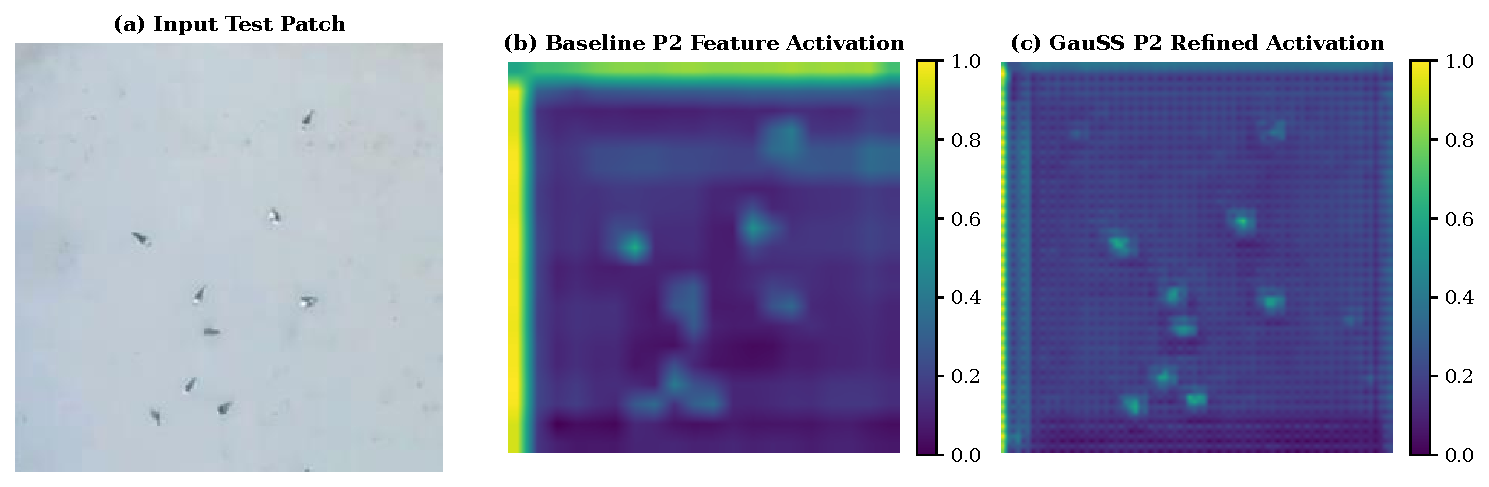
\includegraphics[width=\linewidth]{figures/14_p2_feature_activation_energy.pdf}
    \caption{\textbf{Stride-4 ($P2$) Feature Activation ($L_2$ norm)}: Baseline features dissipate energy across broad water surfaces, whereas GauSS concentrates activation energy around ground-truth targets.}
    \label{fig:p2_activation}
  \end{minipage}\hfill
  \begin{minipage}{0.48\textwidth}
    \centering
    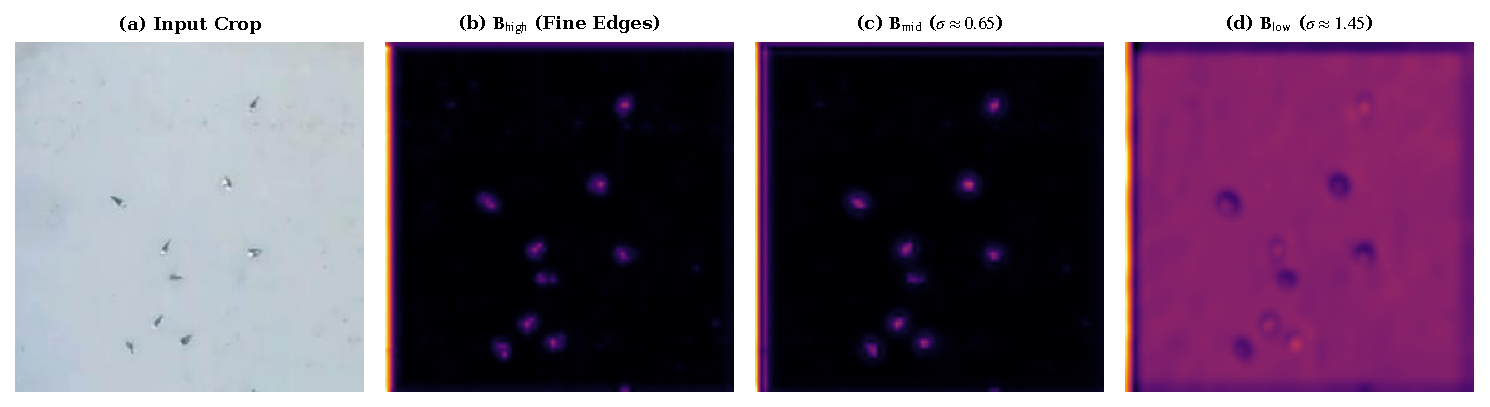
\includegraphics[width=\linewidth]{figures/15_gaussian_band_decomposition.pdf}
    \caption{\textbf{Frequency Band Decomposition}: $\mathbf{B}_{\text{high}}$ captures sharp edges; $\mathbf{B}_{\text{mid}}$ responds strongly to $8\text{--}12\text{ px}$ targets; $\mathbf{B}_{\text{low}}$ provides structural context.}
    \label{fig:band_decomp}
  \end{minipage}
\end{figure*}

\begin{figure*}[t]
  \centering
  \begin{minipage}{0.48\textwidth}
    \centering
    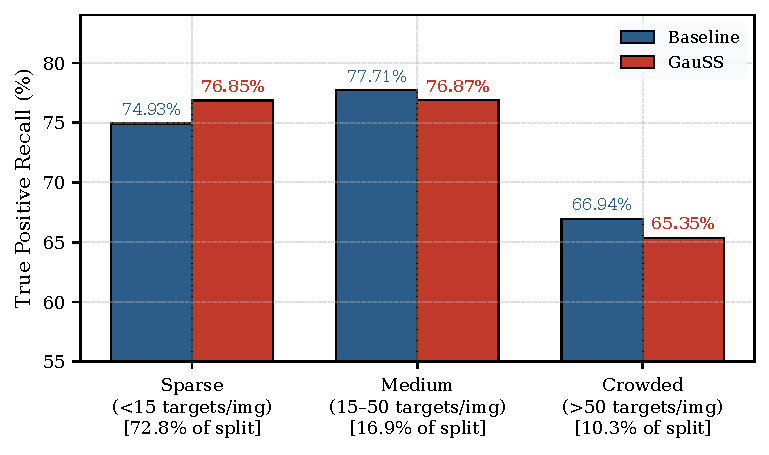
\includegraphics[width=\linewidth]{figures/06_tinyperson_density_recall.pdf}
    \caption{\textbf{Recall Stratification by Scene Density}: GauSS achieves higher recall in sparse scenes ($+1.92\text{ pp}$), which represent $72.8\%$ of maritime operations.}
    \label{fig:density}
  \end{minipage}\hfill
  \begin{minipage}{0.48\textwidth}
    \centering
    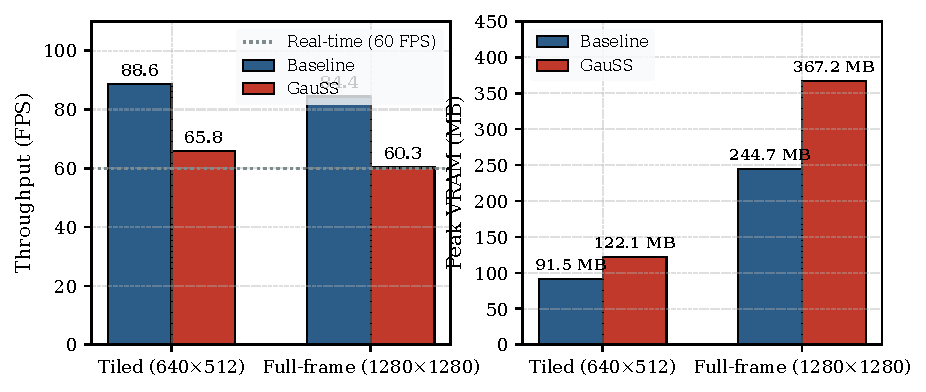
\includegraphics[width=\linewidth]{figures/04_hardware_efficiency.pdf}
    \caption{\textbf{Hardware Profile on NVIDIA A10G}: Latency per tile is $15.19\text{ ms}$ ($65.8\text{ FPS}$) for GauSS vs. $11.28\text{ ms}$ ($88.6\text{ FPS}$) for baseline. Peak VRAM in tiled mode is $122.1\text{ MB}$.}
    \label{fig:hardware}
  \end{minipage}
\end{figure*}

\subsection{Qualitative Analysis and Feature Interpretability}
\label{sec:qualitative_analysis}
To examine the internal representations of GauSS, we inspect four qualitative analyses directly extracted from 150-epoch checkpoints on TinyPerson:
\begin{itemize}
    \item \textbf{Microscopic Detection} (Figure~\ref{fig:qualitative_detections}): In an offshore swimmer cluster containing 6 tiny ground-truth instances, the baseline retains 2 detections at $\ge 0.20$ confidence while GauSS retains 10 at the same threshold, covering the cluster with confidences $0.31$--$0.44$ (frame-level totals: 12 vs.~21).
    \item \textbf{Sea-Clutter Suppression} (Figure~\ref{fig:sea_clutter}): On a wave crest containing no ground truth, the baseline emits one $0.60$-confidence false alarm while GauSS reports none; saliency gating on the low-band context ($(1.0 - 0.5 \mathbf{M}_{\text{sal}})$, Eq.~\ref{eq:saliency_att}) attenuates such background textures.
    \item \textbf{Stride-4 Energy Concentration} (Figure~\ref{fig:p2_activation}): The $L_2$ norm heatmap ($\|\mathbf{F}\|_{L_2}$) shows that baseline activations diffuse broadly across waves, whereas GauSS focuses energy tightly on genuine targets.
    \item \textbf{Band Decomposition} (Figure~\ref{fig:band_decomp}): Visualizing $\{\mathbf{B}_{\text{high}}, \mathbf{B}_{\text{mid}}, \mathbf{B}_{\text{low}}\}$ demonstrates that $\mathbf{B}_{\text{high}}$ isolates high-frequency noise, $\mathbf{B}_{\text{mid}}$ responds to target boundaries, and $\mathbf{B}_{\text{low}}$ models global context.
\end{itemize}

\subsection{Density-Stratified Evaluation}
\label{sec:density_stratified}
Test images are stratified into three density tiers based on ground-truth target counts (Figure~\ref{fig:density}): sparse ($<15$ targets, $72.8\%$ of frames), medium ($15\text{--}50$ targets, $16.9\%$), and crowded ($>50$ targets, $10.3\%$).
\begin{itemize}
    \item \textit{Sparse ($<15$ targets)}: GauSS improves recall from $74.93\%$ to $76.85\%$ ($+1.92\text{ pp}$).
    \item \textit{Medium ($15\text{--}50$ targets)}: GauSS achieves $76.87\%$ vs. $77.71\%$ ($-0.84\text{ pp}$).
    \item \textit{Crowded ($>50$ targets)}: GauSS recall is $65.35\%$ vs. $66.94\%$ ($-1.59\text{ pp}$). In dense clusters, greedy NMS with fixed thresholds~\cite{neubeck2006nms,bodla2017softnms} can suppress adjacent micro-boxes.
\end{itemize}

\subsection{Hardware Profiling and Throughput Analysis}
\label{sec:hardware_profile}
Table~\ref{tab:hardware_bench} and Figure~\ref{fig:hardware} detail profiling on an NVIDIA A10G GPU ($24\text{GB}$ VRAM, FP16, batch size 1, 25 warmup, 100 timed iterations):
\begin{itemize}
    \item \textbf{Complexity}: GauSS adds $0.51\text{ GFLOPs}$ ($+6.7\%$) in tiled mode ($640 \times 512$: $7.62$ vs. $8.13\text{ GFLOPs}$) and $2.02\text{ GFLOPs}$ ($+6.3\%$) in full-frame mode ($31.97$ vs. $33.99\text{ GFLOPs}$).
    \item \textbf{Throughput}: Single-tile latency is $15.19\text{ ms}$ ($65.8\text{ FPS}$) for GauSS vs. $11.28\text{ ms}$ ($88.6\text{ FPS}$) for baseline. Full-frame latency is $16.58\text{ ms}$ ($60.3\text{ FPS}$) vs. $11.85\text{ ms}$ ($84.4\text{ FPS}$).
    \item \textbf{Latency-to-FLOP Overhead}: While FLOPs increase by only $6.7\%$, latency increases by $+34.7\%$ in tiled mode and $+39.9\%$ in full-frame mode. This discrepancy stems from memory-bandwidth bottlenecks in depthwise separable convolutions, multi-branch routing, and sub-pixel reorganization ($\text{PixelShuffle}/\text{PixelUnshuffle}$), which are latency-bound rather than compute-bound at batch size 1.
    \item \textbf{End-to-End Tiling vs. Full-Frame Throughput}: Because test images have diverse native resolutions (median $3840 \times 2160$ px), slicing generates an average of $23.4$ overlapping tiles ($640 \times 512$). Sequential inference over $23.4$ tiles requires $\sim 355\text{ ms}$ per full capture ($\sim 2.8\text{ FPS}$), while a $1280 \times 1280$ capture yields 9 tiles ($\sim 137\text{ ms} \approx 7.3\text{ FPS}$). Conversely, direct full-frame evaluation ($1280 \times 1280$) achieves $16.58\text{ ms}$ ($\mathbf{60.3\text{ FPS}}$ end-to-end), representing an $8.3\times$ speedup over the 9-tile pipeline. As detailed in Table~\ref{tab:hardware_bench}, full-frame inference retains high overall accuracy ($12.53\%$ $AP_{50}^{\text{all}}$), but tiled slicing yields superior localization on microscopic scale intervals ($9.50\%$ vs. $6.90\%$ $AP_{50}^{\text{tiny2}}$) by preserving native sub-pixel detail.
    \item \textbf{VRAM}: Peak VRAM is $122.1\text{ MB}$ in tiled mode and $367.2\text{ MB}$ in full-frame mode.
\end{itemize}

\begin{table*}[t]
\centering
\small
\setlength{\tabcolsep}{6pt}
\caption{\textbf{Comprehensive Hardware and Accuracy Trade-Off: Tiled ($640 \times 512$) vs. Full-Frame ($1280 \times 1280$)}. Timing is measured on an NVIDIA A10G GPU (FP16, batch size 1). End-to-end frame rate considers the full image slicing and inference pipeline. Accuracy is reported across representative scale bins.}
\label{tab:hardware_bench}
\begin{tabular*}{\textwidth}{@{\extracolsep{\fill}}llccccc@{}}
\toprule
\textbf{Mode} & \textbf{Model} & \textbf{Params} & \textbf{Latency / FPS} & \textbf{End-to-End FPS} & \textbf{$AP_{50}^{\text{all}}$} & \textbf{$AP_{50}^{\text{tiny2}}$} \\
\midrule
\multirow{2}{*}{Tiled ($640 \times 512$)}     & Baseline & 2.52M & 11.28 ms / 88.6 & 3.8 -- 9.8 FPS$^\dagger$ & 11.95\% & 6.90\% \\
                                              & GauSS    & 2.55M & 15.19 ms / 65.8 & 2.8 -- 7.3 FPS$^\dagger$ & \textbf{12.94\%} & \textbf{9.50\%} \\
\midrule
\multirow{2}{*}{Full-Frame ($1280 \times 1280$)} & Baseline & 2.52M & 11.85 ms / 84.4 & 84.4 FPS & 12.43\% & 9.90\% \\
                                              & GauSS    & 2.55M & 16.58 ms / 60.3 & \textbf{60.3 FPS} & 12.53\% & 9.60\% \\
\bottomrule
\end{tabular*}
\vspace{1pt}
\raggedright \footnotesize $^\dagger$Range reflects full image resolutions: $\sim 2.8\text{ FPS}$ on high-resolution median ($3840 \times 2160$, 23.4 tiles) up to $\sim 7.3\text{ FPS}$ on standard $1280 \times 1280$ images (9 tiles), sequential without pipeline parallelization.
\end{table*}

\subsection{Multi-Class Transfer Adaptation on VisDrone}
To test cross-domain transfer, 150-epoch checkpoints were fine-tuned on VisDrone-DET~\cite{zhu2021visdrone} for 10 epochs ($\text{lr}_0 = 0.001$, Table~\ref{tab:visdrone_eval} and Figure~\ref{fig:visdrone_class}). On validation, GauSS reaches $25.31\%$ $mAP_{50}$ (vs. $25.64\%$ baseline, $-0.33\text{ pp}$). On test-dev, GauSS achieves $20.33\%$ $mAP_{50}$ (vs. $20.81\%$, $-0.48\text{ pp}$). GauSS exhibits slight improvements on Truck ($+1.22\text{ pp}$ val, $+0.80\text{ pp}$ test-dev) and Pedestrian ($+0.16\text{ pp}$ val). These results demonstrate comparable transfer performance, indicating that inductive priors optimized for maritime scale-space filtering do not degrade general drone detection.

\begin{figure}[t]
  \centering
  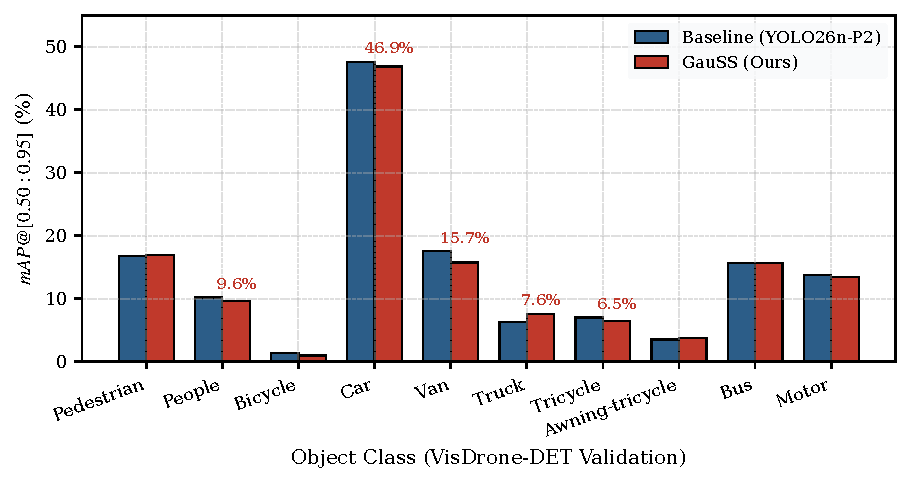
\includegraphics[width=\linewidth]{figures/05_visdrone_per_class_val.pdf}
  \caption{\textbf{Transfer Adaptation on VisDrone-DET (10 Epochs)}: Per-class $mAP@[0.50:0.95]$ on validation split across 10 categories.}
  \label{fig:visdrone_class}
\end{figure}

\begin{table}[t]
\centering
\small
\setlength{\tabcolsep}{5pt}
\caption{\textbf{Transfer Adaptation on VisDrone-DET} after 10 epochs. Evaluation is computed under standard VisDrone evaluation protocols.}
\label{tab:visdrone_eval}
\begin{tabular}{lcccc}
\toprule
\textbf{Split / Metric} & \textbf{Baseline} & \textbf{GauSS} & \textbf{$\Delta$} \\
\midrule
Val: $mAP_{50}$        & 25.64\% & 25.31\% & $-$0.33 pp \\
Val: $mAP_{50:95}$     & 13.97\% & 13.70\% & $-$0.27 pp \\
Val: Truck AP          & 6.36\%  & 7.58\%  & $+$1.22 pp \\
Val: Pedestrian AP     & 16.76\% & 16.92\% & $+$0.16 pp \\
\midrule
Test-dev: $mAP_{50}$   & 20.81\% & 20.33\% & $-$0.48 pp \\
Test-dev: $mAP_{50:95}$& 11.07\% & 10.78\% & $-$0.29 pp \\
Test-dev: Truck AP     & 3.69\%  & 4.49\%  & $+$0.80 pp \\
\bottomrule
\end{tabular}
\end{table}

\begin{figure*}[t]
  \centering
  \begin{minipage}{0.48\textwidth}
    \centering
    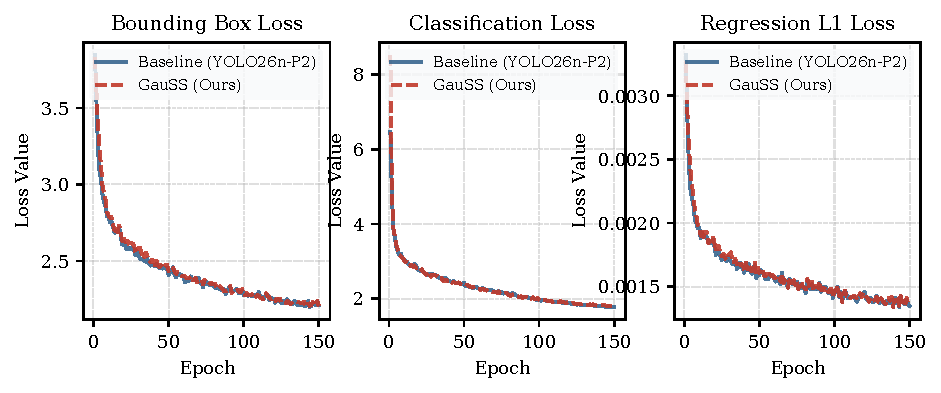
\includegraphics[width=\linewidth]{figures/07_training_loss_convergence.pdf}
    \caption{\textbf{Training Loss Convergence across 150 Epochs}: Box loss, classification loss, and $\ell_1$ loss profiles show steady optimization.}
    \label{fig:train_loss}
  \end{minipage}\hfill
  \begin{minipage}{0.48\textwidth}
    \centering
    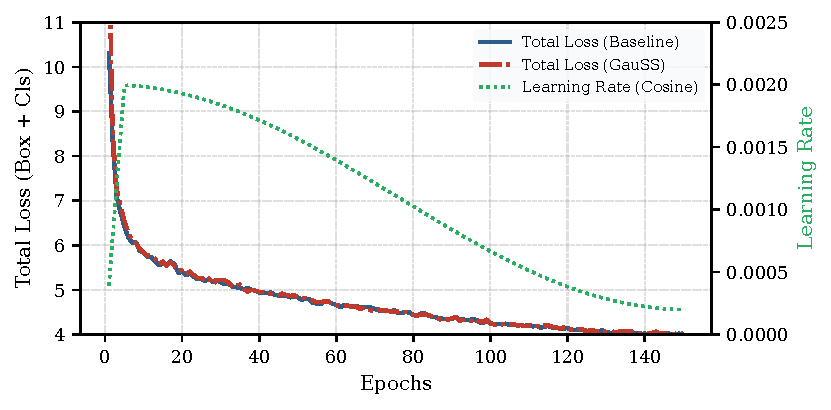
\includegraphics[width=\linewidth]{figures/08_training_total_loss_lr.pdf}
    \caption{\textbf{Total Loss and Cosine Learning Rate Schedule}: Total loss converges smoothly under cosine decay.}
    \label{fig:train_lr}
  \end{minipage}
\end{figure*}

\section{Discussion, Limitations, and Ethical Impact}
\label{sec:discussion}
Figures~\ref{fig:train_loss} and~\ref{fig:train_lr} indicate smooth optimization convergence across 150 epochs. Below we synthesize key limitations, threats to validity, and broader impacts:
\begin{enumerate}
    \item \textbf{Strict-Threshold Localization ($AP_{75}$)}: While GauSS improves $AP_{50}^{\text{all}}$ by $+0.98\text{ pp}$, strict-threshold precision remains very low ($AP_{75} = 1.40\%$ vs. $1.28\%$). Targets spanning only $2\text{--}8$ pixels contain few unambiguous boundary pixels; minute coordinate offsets of 1--2 pixels trigger severe relative IoU drops below $0.75$, demonstrating the fundamental difficulty of high-precision bounding box localization without sub-pixel offset heads.
    \item \textbf{Single-Seed Variance and Bin Fluctuations}: Models were evaluated from single scratch runs per configuration. As shown in Table~\ref{tab:main_tinyperson}, cross-epoch trajectories exhibit non-trivial shifts (e.g., $tiny1$ gain diminishes from $+1.23\text{ pp}$ at 50e to $+0.46\text{ pp}$ at 150e, while $reasonable$ delta shifts from $-1.15\text{ pp}$ to $+0.72\text{ pp}$). Small variations (such as the $-0.14\text{ pp}$ change in $tiny3$) should therefore be treated with caution until multi-seed bootstrap confidence intervals across video sequences are evaluated.
    \item \textbf{End-to-End Tiling vs. Deployment Trade-Off}: While per-tile latency exceeds $60\text{ FPS}$ ($15.19\text{ ms}$), full image slicing produces $23.4$ tiles on native high-resolution images, dropping sequential throughput to $\sim 2.8\text{ FPS}$ ($\sim 7.3\text{ FPS}$ on $1280 \times 1280$). Direct full-frame inference restores $60.3\text{ FPS}$ real-time throughput ($16.58\text{ ms}$), offering an $8.3\times$ speedup at the cost of diminished microscopic gain ($+0.10\text{ pp}$ vs. $+0.98\text{ pp}$ on $AP_{50}^{\text{all}}$).
    \item \textbf{Cross-Domain Generalization}: On VisDrone-DET, fine-tuning GauSS yields $25.31\%$ validation $mAP_{50}$ (vs. $25.64\%$ baseline, $-0.33\text{ pp}$) and $20.33\%$ test-dev $mAP_{50}$ (vs. $20.81\%$, $-0.48\text{ pp}$). While truck and pedestrian categories show slight positive deltas, overall transfer is comparable but marginally lower, indicating that scale-space inductive biases designed for maritime sea clutter do not automatically transfer to dense terrestrial urban traffic.
    \item \textbf{Ethical and Societal Implications}: Aerial tiny person detection serves critical humanitarian goals in maritime search and rescue. However, UAV-based person detection can be dual-use for unauthorized surveillance. Deployment should adhere to strict privacy safeguards and regulatory frameworks.
\end{enumerate}

\section{Conclusion}
\label{sec:conclusion}
We presented \textbf{GauSS}, a scale-space-inspired module for stride-4 feature refinement in nano-scale tiny object detection. By combining learnable Gaussian filtering, frequency band decomposition, and spatial routing, GauSS improves $AP_{50}^{\text{all}}$ by $+0.98\text{ pp}$ and $AP_{50}^{\text{tiny2}}$ by $+2.59\text{ pp}$ on TinyPerson with $+34{,}666$ parameters ($+1.38\%$). On VisDrone, transfer performance is comparable but slightly lower than the baseline. Future work includes extensive parameter-matched ablations against standard convolutions and attention mechanisms, multi-seed variance analysis, kernel fusion for latency reduction, and edge evaluation on embedded Jetson platforms.

{\small
\bibliographystyle{ieee}
\bibliography{references}
}

\end{document}
